%%%%%%%%%%%%%%%%%%%%%%%%%%%%%%%%%%%%

\section{Case study: Gender discrimination}

%%%%%%%%%%%%%%%%%%%%%%%%%%%%%%%%%%%%

\subsection{Study description and data}

%%%%%%%%%%%%%%%%%%%%%%%%%%%%%%%%%%%%

\begin{frame}
\frametitle{Gender discrimination}

\begin{itemize}

\item In 1972, as a part of a study on gender discrimination, 48 male bank supervisors were each given the same personnel file and asked to judge whether the person should be promoted to a branch manager job that was described as ``routine". 

\item The files were identical except that half of the supervisors had files showing the person was male while the other half had files showing the person was female.

\item It was randomly determined which supervisors got ``male" applications and which got ``female" applications.  

\item Of the 48 files reviewed, 35 were promoted. 

\item The study is testing whether females are unfairly discriminated against.  
\end{itemize}

\dq{Is this an observational study or an experiment?} \soln{\onslide<2->{Experiment}}

\ct{B.Rosen and T. Jerdee (1974), ``Influence of sex role stereotypes on personnel decisions", J.Applied Psychology, 59:9-14.}

\end{frame}


%%%%%%%%%%%%%%%%%%%%%%%%%%%%%%%%%%%%

\begin{frame}
\frametitle{Data}

\dq{At a first glance, does there appear to be a relatonship between promotion and gender?}

\begin{center}
\begin{tabular}{ll  cc c} 
  		&				& \multicolumn{2}{c}{\textit{Promotion}} \\
\cline{3-4}
							&			& Promoted	& Not Promoted 	& Total	\\
\cline{2-5}
\multirow{2}{*}{\textit{Gender	}}	&Male 		& 21	 	& 3		& 24 	\\
							&Female		& 14	 	& 10 	 	& 24 \\
\cline{2-5}
							&Total		& 35		& 13		& 48 \\
\end{tabular}
\end{center}

\pause

\textbf{\% of males promoted: $21 / 24 = 0.875$} \\
\textbf{\% of females promoted: $14 / 24 = 0.583$}

\end{frame}

%%%%%%%%%%%%%%%%%%%%%%%%%%%%%%%%%%%%

\begin{frame}
\frametitle{Practice}

\pq{We saw a difference of almost 30\% (29.2\% to be exact) between the proportion of male and female files that are promoted. Based on this information, which of the below is true?}

\begin{enumerate}[(a)]

\item If we were to repeat the experiment we will definitely see that more female files get promoted. This was a fluke.

\item Promotion is dependent on gender, males are more likely to be promoted, and hence there is gender discrimination against women in promotion decisions. \soln{\only<2>{\red{Maybe}}}

\item The difference in the proportions of promoted male and female files is due to chance, this is not evidence of gender discrimination against women in promotion decisions. \soln{\only<2>{\red{Maybe}}}

\item Women are less qualified than men, and this is why fewer females get promoted.

\end{enumerate}

\end{frame}

%%%%%%%%%%%%%%%%%%%%%%%%%%%%%%%%%%%%

\subsection{Competing claims}

%%%%%%%%%%%%%%%%%%%%%%%%%%%%%%%%%%%%%

\begin{frame}
\frametitle{Two competing claims}

\begin{enumerate}

\item ``There is nothing going on." \\
Promotion and gender are \hl{independent}, no gender discrimination, observed difference in proportions is simply due to chance. $\rightarrow$ \hl{Null hypothesis}

\pause

\item ``There is something going on." \\
Promotion and gender are \hl{dependent}, there is gender discrimination, observed difference in proportions is not due to chance. $\rightarrow$ \hl{Alternative hypothesis}

\end{enumerate}

\end{frame}

%%%%%%%%%%%%%%%%%%%%%%%%%%%%%%%%%%%%

\begin{frame}
\frametitle{A trial as a hypothesis test}

\twocol{0.5}{0.5}
{
\begin{itemize}

\item Hypothesis testing is very much like a court trial.

\item $H_0$: Defendant is innocent \\
$H_A$: Defendant is guilty

\item We then present the evidence - collect data.

\end{itemize}
}
{
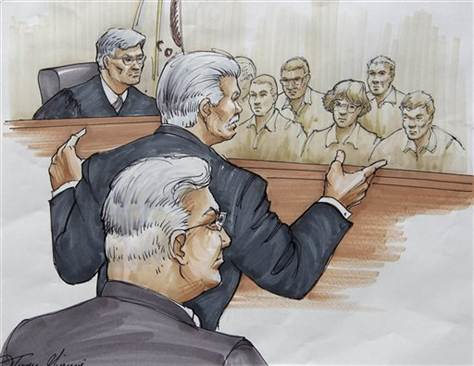
\includegraphics[width=\textwidth]{1-8_gender_discrimination/figures/trial}
}

\begin{itemize}

\item Then we judge the evidence - ``Could these data plausibly have happened by chance if the null hypothesis were true?"
\begin{itemize}
\item If they were very unlikely to have occurred, then the evidence raises more than a reasonable doubt in our minds about the null hypothesis.
\end{itemize}

\item Ultimately we must make a decision. How unlikely is unlikely?

\end{itemize}

\ct{Image from \webURL{http://www.nwherald.com/_internal/cimg!0/oo1il4sf8zzaqbboq25oevvbg99wpot}.}

\end{frame}

%%%%%%%%%%%%%%%%%%%%%%%%%%%%%%%%%%%%%

\begin{frame}
\frametitle{A trial as a hypothesis test (cont.)}

\begin{itemize}

\item If the evidence is not strong enough to reject the assumption of innocence, the jury returns with a verdict of ``not guilty".
\begin{itemize}
\item The jury does not say that the defendant is innocent, just that there is not enough evidence to convict.
\item The defendant may, in fact, be innocent, but the jury has no way of being sure.
\end{itemize}

\item Said statistically, we fail to reject the null hypothesis.
\begin{itemize}
\item We never declare the null hypothesis to be true, because we simply do not know whether it's true or not.
\item Therefore we never ``accept the null hypothesis".
\end{itemize}

\end{itemize}

\end{frame}

%%%%%%%%%%%%%%%%%%%%%%%%%%%%%%%%%%%%%

\begin{frame}
\frametitle{A trial as a hypothesis test (cont.)}

\begin{itemize}

\item In a trial, the burden of proof is on the prosecution.

\item In a hypothesis test, the burden of proof is on the unusual claim.

\item The null hypothesis is the ordinary state of affairs (the status quo), so it's the alternative hypothesis that we consider unusual and for which we must gather evidence.

\end{itemize}

\end{frame}

%%%%%%%%%%%%%%%%%%%%%%%%%%%%%%%%%%%%%

\begin{frame}
\frametitle{Recap: hypothesis testing framework}

\begin{itemize}
\item We start with a \hl{null hypothesis ($H_0$)} that represents the status quo.
\item We also have an \hl{alternative hypothesis ($H_A$)} that represents our research question, i.e. what we're testing for.
\item We conduct a hypothesis test under the assumption that the null hypothesis is true, either via simulation (today) or theoretical methods (later in the course).
\item If the test results suggest that the data do not provide convincing evidence for the alternative hypothesis, we stick with the null hypothesis. If they do, then we reject the null hypothesis in favor of the alternative.
\end{itemize}

\end{frame}

%%%%%%%%%%%%%%%%%%%%%%%%%%%%%%%%%%%%

\subsection{Testing via simulation}

%%%%%%%%%%%%%%%%%%%%%%%%%%%%%%%%%%%%%

\begin{frame}
\frametitle{Simulating the experiment...}

... under the assumption of independence, i.e. leave things up to chance. \\

\vspace{0.5cm}

If results from the simulations based on the \hl{chance model} look like the data, then we can determine that the difference between the proportions of promoted files between males and females was simply \hl{due to chance} (promotion and gender are independent). \\

\vspace{0.5cm}

If the results from the simulations based on the chance model do not look like the data, then we can determine that the difference between the proportions of promoted files between males and females was not due to chance, but \hl{due to an actual effect of gender} (promotion and gender are dependent).

\end{frame}


%%%%%%%%%%%%%%%%%%%%%%%%%%%%%%%%%%%%%